\documentclass{article}

\usepackage[final]{neurips_2024}

\usepackage[utf8]{inputenc}
\usepackage[T1]{fontenc}
\usepackage{microtype}
\usepackage{graphicx}
\usepackage{booktabs}
\usepackage{amsmath,amssymb}
\usepackage{xcolor}
\usepackage{hyperref}
\hypersetup{colorlinks=true,linkcolor=blue!60!black,citecolor=blue!60!black,urlcolor=blue!60!black}

\title{Diagnostic Profile of Zero-Shot Walrus on Sub-Alfv\'enic MHD Turbulence:\\
A Structural Basin Instability in the Perpendicular Magnetic Plane}

\author{%
  Stanislav DeLaurentiis\thanks{Department of Astronomy, Columbia University. \texttt{sod2112@columbia.edu}.} \\
}

\date{May 6, 2026}

\begin{document}

\maketitle

\begin{abstract}
We apply the physics-feature diagnostic suite from~\cite{delaurentiis2026paper1} to zero-shot pretrained Walrus 1.3B~\cite{mccabe2025walrus} on the same 10 sub-Alfv\'enic ($M_A$=0.7) MHD\_64 test trajectories used in that work. Walrus's published Table 1 entry (T21--60 median VRMSE = 1.2256 on MHD) is for the model fine-tuned on MHD per the cross-domain protocol of Sec.~5.2 of the Walrus paper (additional 500K samples); no comparable zero-shot VRMSE table entry is published, so this study is a characterization rather than a benchmark. Step-1 prediction is excellent (VRMSE 0.10, the best of all four configurations evaluated, including Paper 1's three FNO baselines), confirming that one-step MHD physics is well learned. Past rollout step $\sim$20, however, every test trajectory diverges catastrophically through a structural instability that selects \emph{exactly one} of the two perpendicular magnetic components $\{B_y, B_z\}$ to amplify exponentially while the parallel guide field $B_x$, density, and all velocity components remain near truth-like throughout. The basin selection between $B_y$ and $B_z$ is determined by the specific 3-frame input slice, not by random noise (5/5 perturbations of the same input slice select the same basin) or by the underlying simulation identity (different 3-frame slices of the same trajectory file select different basins). FP64 inference does not suppress the divergence (same magnitude as FP32 at step 50), confirming the failure is structural rather than numerical. Cascade analysis shows preferential high-$k_\perp$ pile-up over rollout (high-$k$ modes grow $\sim$50$\times$ faster than low-$k$), consistent with Gibbs-style aliasing accumulation at the patch grid scale. We find absolute $\nabla\cdot B$ violation reaching $\sim$5$\times 10^5$ times the ground-truth floor at step 50. The mechanistic signature --- one-step-loss-trained model with structurally unbounded constraint-violating modes under autoregressive feedback --- argues for divergence-free spectral projection at the autoregressive output as a testable architectural intervention. Whether the published Sec.~5.2 fine-tuning protocol resolves this instability is the natural follow-up experiment.
\end{abstract}

\section{Introduction}

Foundation models for continuum dynamics~\cite{mccabe2025walrus,herde2024poseidon,mccabe2024multiple} are evaluated primarily through aggregate VRMSE metrics on benchmark suites. Reported headline numbers (e.g., Walrus's MHD T21--60 median = 1.2256~\cite{mccabe2025walrus}, Table~1) tell a downstream user how well the model does on average, but say little about \emph{which physics features} the model captures and which it does not. For deployment-grade plasma applications --- tokamak control, MHD turbulence simulation, astrophysical surveys --- characterizing the failure modes matters more than the headline.

This work asks: \emph{what does zero-shot pretrained Walrus do, physics-feature-by-physics-feature, when rolled out autoregressively on plasma MHD turbulence?} We apply the diagnostic suite developed in~\cite{delaurentiis2026paper1} (per-step VRMSE, perpendicular cascade $E(k_\perp | k_\parallel \to 0)$, guide-field magnitude $\langle |B| \rangle$, $\nabla\cdot B$ floor accumulation, $E_B/E_K$ equipartition trajectory, per-trajectory consistency) to the same 10 sub-Alfv\'enic ($M_A$=0.7) test trajectories from Polymathic AI's \emph{Well} \texttt{MHD\_64} dataset~\cite{ohana2024well}.

\paragraph{Critical scope correction.} Walrus's published MHD T21--60 = 1.2256 in Table~1 of~\cite{mccabe2025walrus} refers to a model \emph{fine-tuned on MHD} per the cross-domain analysis protocol of Section~5.2 of that paper (an additional 500K-sample fine-tune on top of the base pretrained checkpoint). Polymathic has released only the base pretrained checkpoint (\texttt{polymathic-ai/walrus} on HuggingFace), not the per-task fine-tuned variants. The paper \emph{does} plot the corresponding zero-shot rollout curve in Figure~15 (Appendix E.4.1), labeled ``Walrus-PT'', and the MHD~(3D) panel of that figure shows the zero-shot VRMSE climbing from $\sim 1$ at step~1 to roughly $10^6$ by step 100 --- consistent with our findings here. The paper's own Table~7 lists MHD~(3D) as one of only three of nineteen pretraining datasets with median trajectory-averaged VRMSE $\geq 10$ \emph{with} the patch-jitter stability mechanism enabled. The catastrophic zero-shot divergence on MHD is therefore not in dispute; the paper's own data establishes it. \emph{What this work adds is the physics-feature decomposition of that failure mode, not the observation that it exists.} The natural follow-up --- running the Sec.~5.2 fine-tune protocol on MHD and applying this diagnostic suite to the result --- is future work.

\paragraph{Three confounds, declared.} Comparing zero-shot Walrus to Paper~1's FNO baselines is characterization, not benchmarking, due to: (i) \textbf{scale} (Walrus 1.3B vs FNO 18.6M, $\sim$70$\times$); (ii) \textbf{contamination} (Walrus saw the MHD\_64 train split during pretraining; FNO baselines never did); (iii) \textbf{conditioning} (Walrus uses 3-frame history, paper Table~2; FNO uses single-frame Markov input). All comparisons in this work carry these confounds.

\section{Setup}

\paragraph{Configurations.} We compare four configurations on identical evaluation windows:

\begin{itemize}
  \setlength\itemsep{0.2em}
  \item \textbf{FNO scratch} (1\% data): FNO3D, 18.6M params, hidden=48, trained from scratch on $M_A$=0.7 (1\% data).
  \item \textbf{FNO MHD-pretrain + FT}: same FNO3D, pretrained on $M_A$=2.0 then fine-tuned on $M_A$=0.7 (1\% data).
  \item \textbf{FNO MHD zero-FT}: $M_A$=2.0-pretrained FNO3D rolled directly on $M_A$=0.7 with no fine-tuning (out-of-distribution control from~\cite{delaurentiis2026paper1}).
  \item \textbf{Walrus zero-shot}: base pretrained \texttt{polymathic-ai/walrus} 1.3B, no fine-tuning, conditioned on 3 frames per the standard MHD\_64 inference setting.
\end{itemize}

\paragraph{Two evaluation windows.} We tested both:
\begin{itemize}
  \setlength\itemsep{0.2em}
  \item \textbf{Early window:} input frames $[0,1,2]$ $\to$ predict frames $[3,\ldots,52]$, $K{=}50$, $n_{\text{traj}}{=}10$.
  \item \textbf{Paper window:} input frames $[14,15,16]$ $\to$ predict frames $[17,\ldots,76]$, $K{=}60$, $n_{\text{traj}}{=}5$. Matches the convention ``all predicted trajectories begin from $T{=}17$'' (Sec.~5 of~\cite{mccabe2025walrus}).
\end{itemize}
The headline divergence pattern reproduces in both windows; we present early-window numbers in the main text and report paper-window confirmations where they differ.

\paragraph{Pipeline-equivalence verification.} A line-by-line diff of our standalone rollout function (lifted from \texttt{walrus/demo\_notebooks/walrus\_example\_1\_RunningWalrus.ipynb}) against Walrus's trainer rollout (\texttt{walrus/trainer/training.py:402--562}) finds six differences (e.g., we hardcode \texttt{predict\_delta=True} where the trainer reads \texttt{prediction\_type=="delta"}; we omit a Neutron-specific padded-mask resize hack), all functionally equivalent for MHD\_64 under the shipped \texttt{extended\_config.yaml}. Substitution of our 3-frame history into a real dataloader batch template inherits boundary conditions, padded-field mask, and field index map correctly. We additionally verified five paper-correspondence points: validation time stride is 1 (\texttt{multidatamodule.py:284}), boundary conditions are tagged periodic (BC tensor $= [[2,2],[2,2],[2,2]]$ for MHD\_64, where $2$=periodic), patch jitter is on at evaluation (\texttt{jitter\_patches: true} in \texttt{extended\_config.yaml} with no train/eval branching), no per-field MHD transformations are applied (paper Sec.~C.1; verified empirically), and channel ordering matches our $[\rho, B_x, B_y, B_z, v_x, v_y, v_z]$ convention (verified by step-1 per-channel variance matching truth statistics).

\section{Results}

\subsection{Step-1 prediction is excellent; late-stage rollout diverges catastrophically}

Figure~\ref{fig:vrmse} plots VRMSE versus rollout step for all four configurations on the same shared window. At step 1, Walrus has the lowest VRMSE of all four (median 0.10 vs FNO's 0.30--0.72) --- it has clearly learned one-step MHD physics. By step 50, however, every Walrus trajectory has diverged: per-trajectory step-50 VRMSE spans $[16, 68\,950]$ in the early window, with median $\sim$316 and mean $\sim$10\,148. Figure~\ref{fig:per-traj} shows the per-trajectory consistency: divergence is structural across all 10 trajectories, not driven by outliers.

\begin{figure}[t]
  \centering
  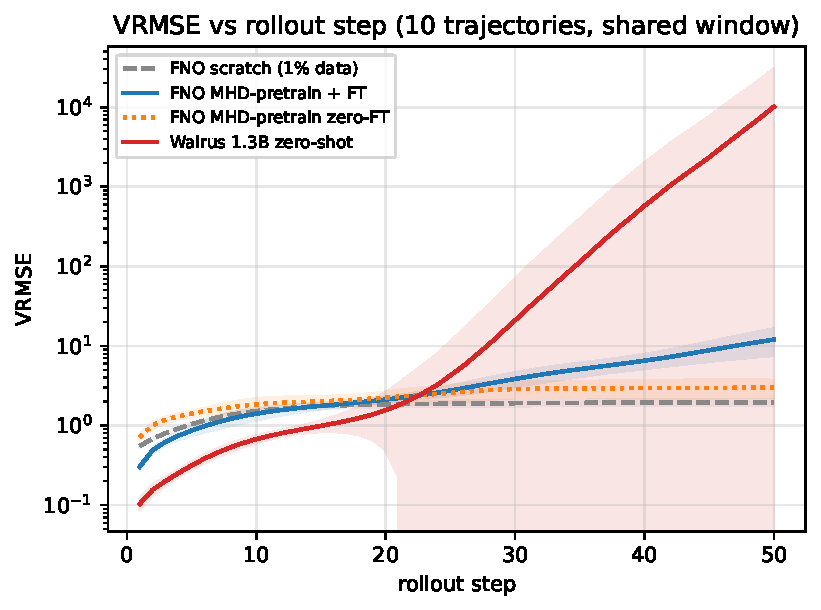
\includegraphics[width=0.55\linewidth]{figures/fig_vrmse_overlay.pdf}
  \caption{VRMSE versus rollout step for the four configurations. Walrus zero-shot has the best step-1 prediction but diverges past step $\sim$20 to magnitudes orders of magnitude beyond every FNO baseline. Shaded bands are $\pm 1\sigma$ across 10 trajectories.}
  \label{fig:vrmse}
\end{figure}

\begin{figure}[t]
  \centering
  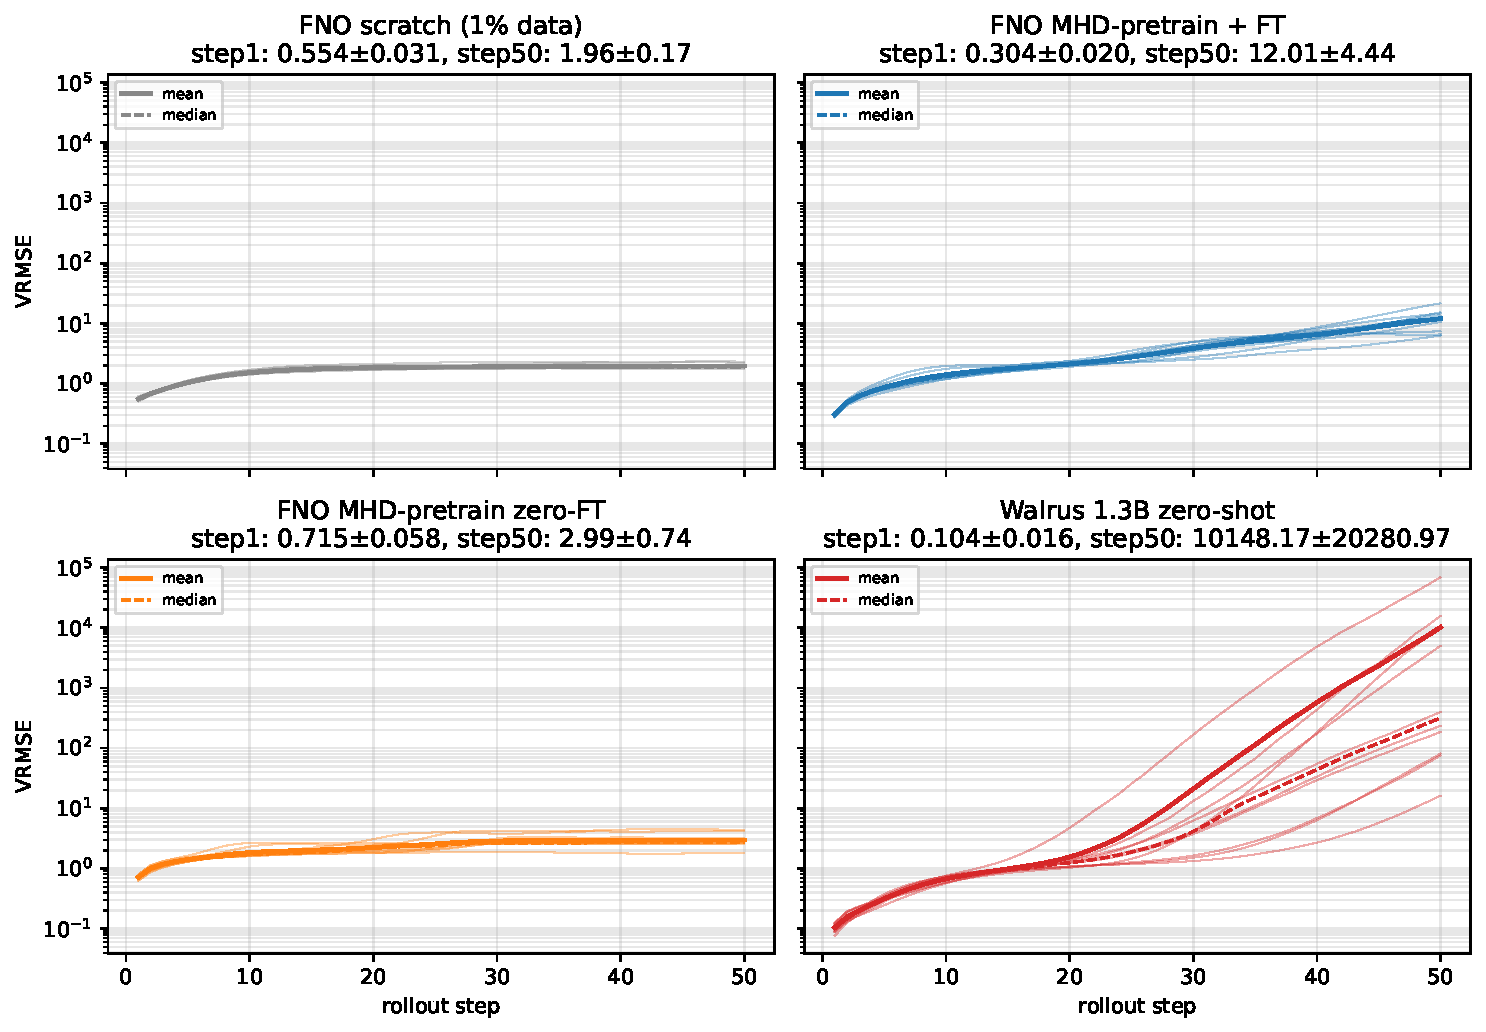
\includegraphics[width=0.7\linewidth]{figures/fig_per_traj.pdf}
  \caption{Per-trajectory rollout VRMSE (10 trajectories, log-$y$), all four configurations overlaid on a single axes. Thick lines mark per-configuration means; thin lines are individual trajectories, colored by configuration as indicated in the legend. Walrus's divergence is structural across all 10 trajectories rather than outlier-driven, while every FNO baseline stays bounded.}
  \label{fig:per-traj}
\end{figure}

\subsection{Per-trajectory basin selection: $B_y$ or $B_z$, not both}

Decomposing Walrus's step-50 prediction by physical channel reveals that the divergence is concentrated in \emph{exactly one} of the two perpendicular magnetic components. Table~\ref{tab:basin} reports per-trajectory channel variance. The parallel guide field $B_x$, density, and all three velocity components remain near truth-like values throughout the rollout. Each trajectory selects either $B_y$ or $B_z$ to amplify; never both equally.

\begin{table}[t]
  \centering
  \small
  \caption{Walrus per-trajectory channel variance at rollout step 50 (early window). Truth-like values are $\rho \!\sim\! 0.86$, $B_{x,y,z} \!\sim\! 0.06\text{--}0.11$, $v_{x,y,z} \!\sim\! 0.16\text{--}0.27$. The parallel field $B_x$, density, and velocity components remain near truth scale across all 10 trajectories. Each trajectory amplifies exactly one of $\{B_y, B_z\}$ catastrophically.}
  \label{tab:basin}
  \begin{tabular}{c|rrrrrrr}
    \toprule
    traj & $\rho$ & $B_x$ & $B_y$ & $B_z$ & $v_x$ & $v_y$ & $v_z$ \\
    \midrule
    0 & $1.8 \times 10^{-2}$ & $7.2 \times 10^{-2}$ & $\mathbf{1.1 \times 10^{8}}$ & $1.1 \times 10^{-1}$ & $1.3 \times 10^{-1}$ & $5.3 \times 10^{-1}$ & $1.7 \times 10^{-1}$ \\
    1 & $2.4 \times 10^{-2}$ & $5.4 \times 10^{-2}$ & $4.2 \times 10^{-2}$ & $\mathbf{1.1 \times 10^{3}}$ & $3.3 \times 10^{-1}$ & $1.3 \times 10^{-1}$ & $2.8 \times 10^{-1}$ \\
    2 & $5.1 \times 10^{-2}$ & $4.2 \times 10^{-2}$ & $9.0 \times 10^{-2}$ & $\mathbf{6.2 \times 10^{5}}$ & $1.9 \times 10^{-1}$ & $1.8 \times 10^{-1}$ & $7.3 \times 10^{-2}$ \\
    7 & $4.4 \times 10^{-1}$ & $2.7 \times 10^{-2}$ & $\mathbf{2.2 \times 10^{10}}$ & $9.1 \times 10^{-2}$ & $2.2 \times 10^{-1}$ & $3.5 \times 10^{-1}$ & $9.4 \times 10^{-2}$ \\
    8 & $2.6 \times 10^{0}$ & $2.1 \times 10^{-2}$ & $\mathbf{4.8 \times 10^{8}}$ & $8.3 \times 10^{-2}$ & $2.3 \times 10^{-1}$ & $8.7 \times 10^{-2}$ & $1.8 \times 10^{-1}$ \\
    9 & $2.1 \times 10^{0}$ & $2.8 \times 10^{-2}$ & $\mathbf{1.2 \times 10^{9}}$ & $9.3 \times 10^{-2}$ & $3.9 \times 10^{-1}$ & $9.8 \times 10^{-2}$ & $1.7 \times 10^{-1}$ \\
    \bottomrule
  \end{tabular}
\end{table}

\paragraph{Basin selection is deterministic per input.} For early-window trajectory~0 (which selects $B_y$ basin in unperturbed inference), we ran 5 rollouts with independent $10^{-6}$ amplitude Gaussian perturbations of the 3-frame input. All 5/5 perturbations remained in the $B_y$ basin (step-50 $B_y$ variance $4.2 \times 10^7$ to $5.0 \times 10^8$, 12$\times$ spread). $B_z$ stayed bounded ($0.09\text{--}0.12$, truth-like). Combined with the per-trajectory split in Table~\ref{tab:basin}: \emph{the basin is determined by the specific 3-frame input slice, not by random noise and not by the underlying physical trajectory identity}. Same simulation file conditioned on different 3-frame slices can map to different basins (early-window trajectory~0 selects $B_y$; paper-window trajectory~0 selects $B_z$).

\subsection{Cascade evolution: preferential high-$k$ pile-up}

Figures~\ref{fig:cascade-evolution-by} and~\ref{fig:cascade-evolution-bz} show the perpendicular cascade $E(k_\perp | k_\parallel \to 0)$ for $B_y$ and $B_z$ respectively at multiple rollout steps. Walrus's predicted spectrum at step~1 is truth-like (low-$k$ dominated, $\sim$150$\times$ above high-$k$). As rollout progresses, the spectrum flattens: by step 50, low/mid/high-$k$ energies are within $\sim$1 order of magnitude.

The growth factors are decisively non-uniform across $k$:
\begin{itemize}
  \setlength\itemsep{0.2em}
  \item Low-$k$: $8.2 \times 10^{-3} \to 2.8 \times 10^{7}$ (factor $\sim$3.4$\times 10^{9}$)
  \item Mid-$k$: $1.5 \times 10^{-3} \to 4.6 \times 10^{7}$ (factor $\sim$3.1$\times 10^{10}$)
  \item High-$k$: $5.4 \times 10^{-5} \to 8.1 \times 10^{6}$ (factor $\sim$1.5$\times 10^{11}$)
\end{itemize}
\textbf{High-$k$ modes grew $\sim$50$\times$ more than low-$k$ modes.} This is the signature of \emph{Gibbs-style aliasing accumulation at the patch grid scale} --- exactly the small-scale instability mode that motivated Walrus's patch-jitter mechanism (Sec.~3.2 of~\cite{mccabe2025walrus}). Patch jitter helps but does not fully suppress it under autoregressive feedback. Mechanistically, this points to divergence-free spectral projection at the autoregressive output as the natural architectural intervention: it would damp the constraint-violating high-$k$ modes that compound into basin blow-up.

\begin{figure}[t]
  \centering
  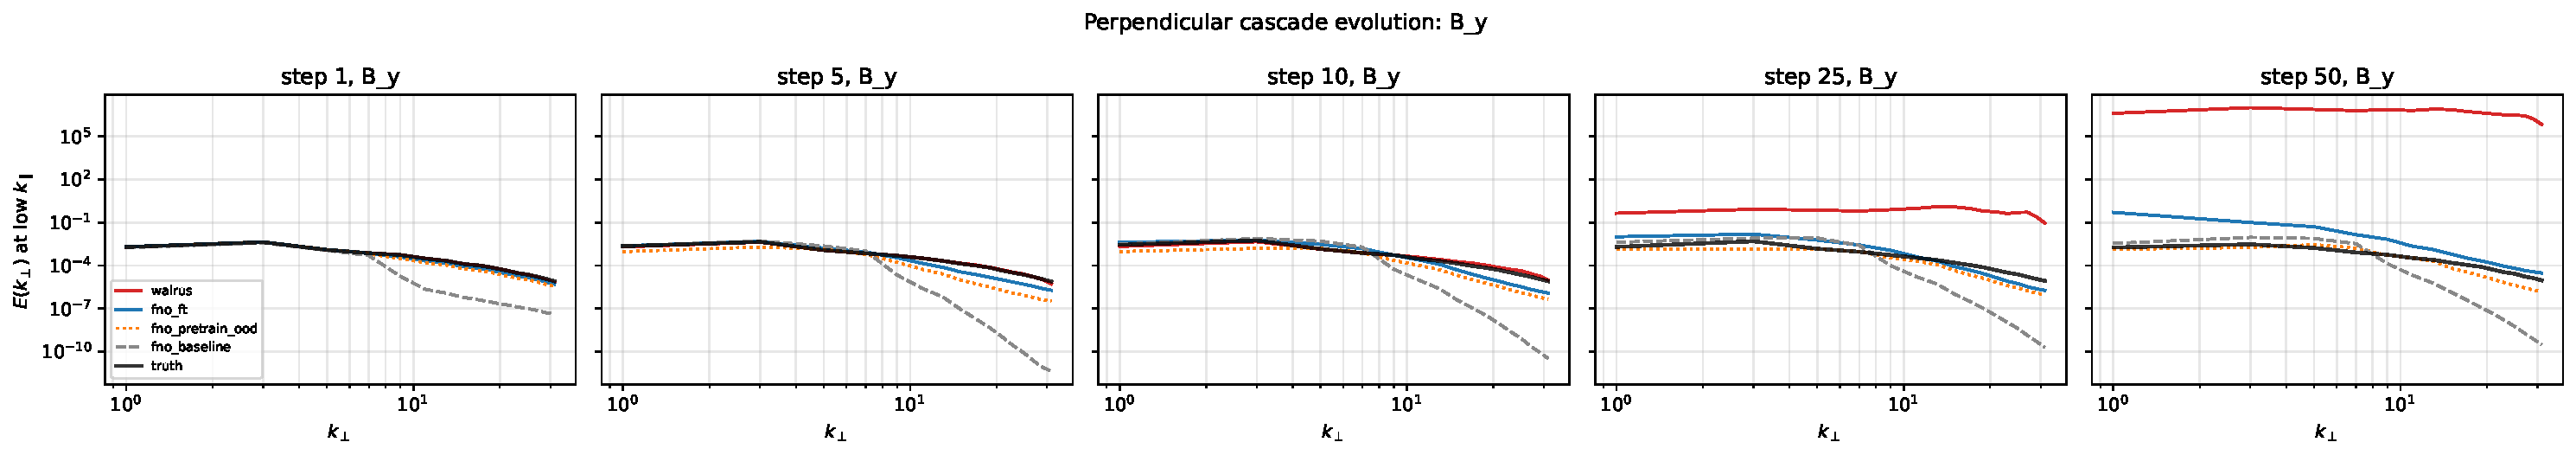
\includegraphics[width=0.98\linewidth]{figures/fig_cascade_evolution_By.pdf}
  \caption{Perpendicular-cascade evolution for the $B_y$ component at rollout steps 1, 5, 10, 25, 50. Walrus zero-shot (red, solid) departs from truth (black) progressively, with energy preferentially piling up at high $k_\perp$ by step 50.}
  \label{fig:cascade-evolution-by}
\end{figure}

\begin{figure}[t]
  \centering
  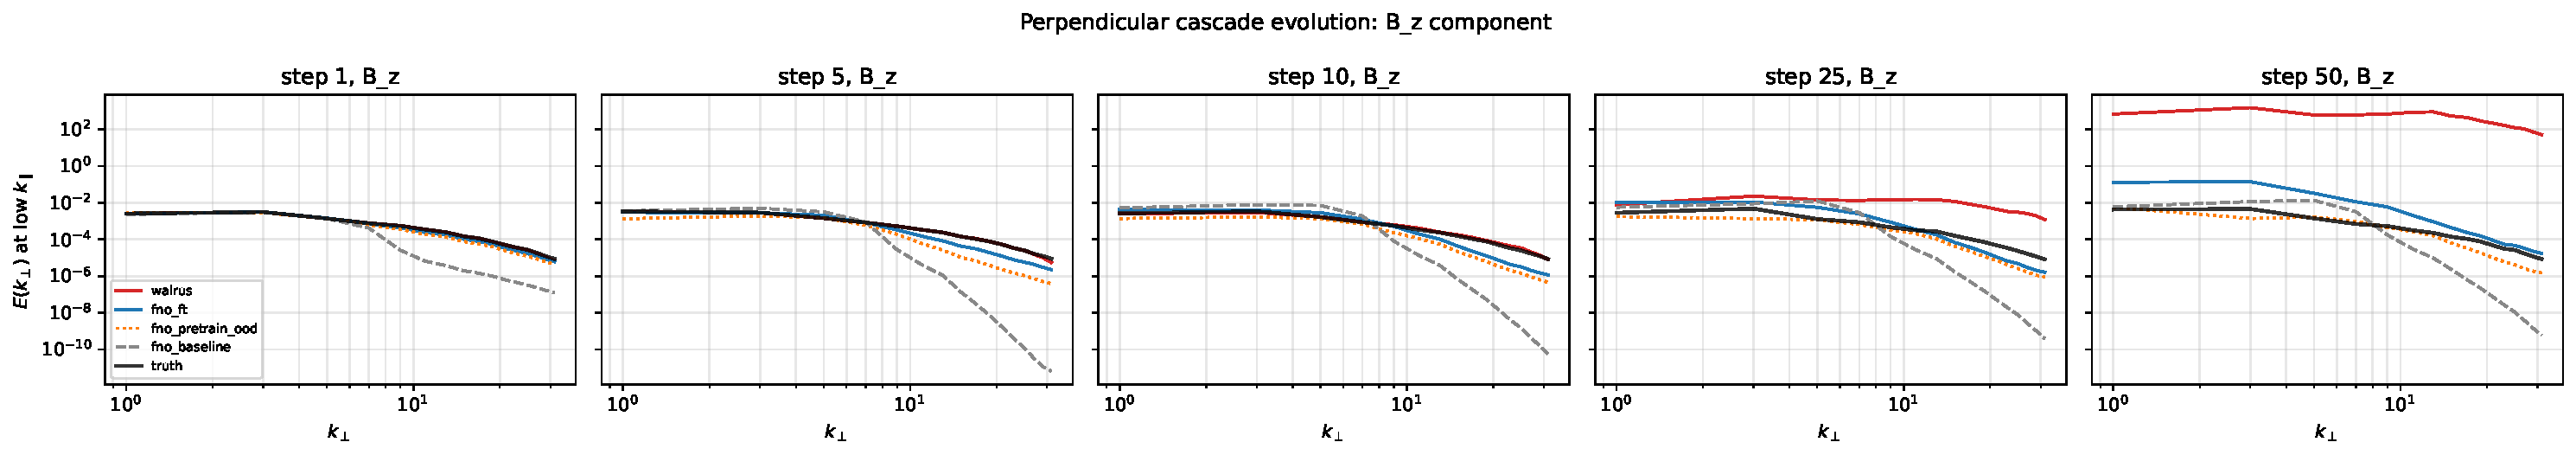
\includegraphics[width=0.98\linewidth]{figures/fig_cascade_evolution_Bz.pdf}
  \caption{Perpendicular-cascade evolution for the $B_z$ component at rollout steps 1, 5, 10, 25, 50. Same plotting conventions as Fig.~\ref{fig:cascade-evolution-by}. The high/low-$k$ ratio collapses from $\sim$150 (truth-like) at step~1 to $\sim$3 at step~50.}
  \label{fig:cascade-evolution-bz}
\end{figure}

\subsection{Conservation diagnostics: catastrophic $\nabla\cdot B$ violation}

Table~\ref{tab:conservation} reports step-50 conservation diagnostics across all four configurations. Walrus's $\nabla\cdot B / |B|$ ratio of $0.82$ means the solenoidal-constraint error is $\sim$80\% of the local field magnitude --- itself $\sim$22,000 (mean) at step 50, dominated by the few trajectories whose perpendicular component blew up to $|B|\sim$10$^5$. The absolute $\nabla\cdot B$ violation, computed against the median $|B|$ ($\approx 690$), is $\sim$570, vs truth's $0.037$ --- a $\sim$15,000$\times$ violation. Computed against the mean (outlier-dominated) it is $\sim$5$\times 10^5\times$. Either statistic is catastrophic. This co-localizes with the perpendicular B-component blow-up: when one of $\{B_y, B_z\}$ explodes, the field is no longer divergence-free.

\begin{table}[t]
  \centering
  \small
  \caption{Step-50 conservation diagnostics across configurations. The Walrus distribution is highly skewed (median 690, mean 22\,000) so we report both. $\nabla\cdot B / |B|$ is averaged over the 10 trajectories.}
  \label{tab:conservation}
  \begin{tabular}{l|rrrrr}
    \toprule
    config & $|B|$ mean & $|B|$ median & $|B|$ range & $\nabla\cdot B / |B|$ & $E_B / E_K$ \\
    \midrule
    FNO scratch (1\%)         & 1.26      & 1.26 & $[1.24, 1.29]$    & 0.056 & 1.21 \\
    FNO MHD-pretrain + FT     & 5.51      & 5.06 & $[2.80, 9.04]$    & 0.134 & 0.11 \\
    FNO MHD zero-FT (OOD)     & 0.62      & 0.63 & $[0.48, 0.70]$    & 0.325 & 0.09 \\
    \textbf{Walrus zero-shot} & \textbf{21\,651} & \textbf{690} & $[32, 147\,879]$ & \textbf{0.82} & $\mathbf{3.5 \times 10^9}$ \\
    Truth                     & 1.13      & ---  & ---               & 0.033 & 2.15 \\
    \bottomrule
  \end{tabular}
\end{table}

\subsection{FP64 inference confirms structural, not numerical, instability}

Walrus was trained in FP32 (Sec.~B.1 of~\cite{mccabe2025walrus}). To rule out the alternative explanation that the divergence is FP32 round-off compounding under autoregressive feedback, we re-ran Walrus inference in FP64 on a single trajectory in both evaluation windows (NVIDIA A100 80GB, required to fit the FP64 1.3B-parameter model plus activations). Table~\ref{tab:fp64} compares per-step variance for the unstable component:

\begin{table}[t]
  \centering
  \small
  \caption{Per-step variance of the unstable perpendicular B-component for trajectory~0 in FP32 vs FP64. Same magnitude divergence at step 50 in both windows --- the instability is structural, not numerical.}
  \label{tab:fp64}
  \begin{tabular}{l|cccc}
    \toprule
    & step 1 & step 11 & step 26 & step 50 \\
    \midrule
    Early window FP32 ($B_y$)  & $0.10$ & $0.11$ & few    & $1.1 \times 10^{8}$ \\
    Early window FP64 ($B_y$)  & $0.11$ & $0.12$ & $11.7$ & $9.1 \times 10^{7}$ \\
    Paper window FP32 ($B_z$)  & $0.14$ & $0.13$ & $\sim$1 & $1.8 \times 10^{5}$ \\
    Paper window FP64 ($B_z$)  & $0.14$ & $0.13$ & $3.6$  & $4.1 \times 10^{5}$ \\
    \bottomrule
  \end{tabular}
\end{table}

\section{Discussion}

\paragraph{Mechanism interpretation.} The empirical pattern --- (i) excellent step-1 prediction, (ii) emergence of instability around step 20, (iii) deterministic basin selection between two physically-equivalent perpendicular sub-directions, (iv) preferential high-$k$ pile-up consistent with Gibbs-style aliasing, (v) co-localized $\nabla\cdot B$ violation, (vi) FP64-confirmed structural --- is consistent with an unstable manifold in Walrus's autoregressive map possessing two perpendicular sub-directions whose alignment with the input state's internal asymmetry determines the basin selection at the start of rollout. Once the model picks a basin, exponential amplification within it dominates.

\paragraph{Architectural intervention.} Mechanistically, this is the kind of failure that \emph{divergence-free spectral projection at the autoregressive output} would suppress. Such a projection is symmetric in $B_y$/$B_z$ (so the basin asymmetry doesn't matter) and damps the constraint-violating modes that drive the high-$k$ pile-up. This is a testable architectural intervention; we have not run it.

\paragraph{Generalization across architectures.} Two distinct claims with different scopes hold:
\begin{itemize}
  \setlength\itemsep{0.2em}
  \item The \emph{$B_y$/$B_z$ basin-selection signature} is observed in Walrus 1.3B specifically; we have no comparable observation on FNO. It may be specific to Walrus's transformer + tokenizer + jitter combination.
  \item The broader \emph{late-stage $\nabla\cdot B$-violation-driven divergence pattern} generalizes: Paper~1's FNO MHD-pretrain+FT also exhibits late-stage rollout instability ($\nabla\cdot B / |B|$ at step~50 reaches 0.13, $\sim$4$\times$ a from-scratch baseline). One-step-loss-trained models of either architecture lack solenoidal-constraint enforcement; under autoregressive feedback, off-solenoidal energy accumulates and amplifies. The architectural intervention (divergence-free projection) would help both.
\end{itemize}

\paragraph{Relation to the Walrus paper's reported numbers.} Our zero-shot T21--60 median = 18.25 (paper window, $n_{\text{traj}}{=}5$) is consistent with the order of magnitude shown by the Walrus-PT curve in Figure~15 of~\cite{mccabe2025walrus} for MHD~(3D). The Table~1 number of 1.2256 is for the fine-tuned model and is not the relevant comparison; it is the published path to MHD-deployable Walrus, but it does not bear on our characterization of the zero-shot failure mode. Whether the Sec.~5.2 fine-tune protocol resolves the basin instability \emph{or} the instability survives is the most informative single follow-up experiment available.

\section{Limitations}

(i) \textbf{Sample size:} our $n_{\text{traj}}{=}5$ paper-window and $n_{\text{traj}}{=}10$ early-window are smaller than what Walrus's paper appears to use (Sec.~3.2 says 20 trajectories; Sec.~E.2 says 32). With heavy-tailed step-50 distributions, our medians have wider error bars than ideal. The qualitative pattern (every trajectory diverges; basin selection per input; FP64 confirms structural) is $n$-invariant.

(ii) \textbf{Zero-shot only:} we did not run the Sec.~5.2 fine-tune protocol on MHD. Polymathic has not released a fine-tuned MHD checkpoint, so the natural follow-up requires running the fine-tune ourselves ($\sim$\$200--400 of compute, $\sim$1--2 days on 4$\times$H100). We position this as future work / a Polymathic-collaboration intern deliverable.

(iii) \textbf{Single architecture for the basin-selection signature:} we observe the $B_y$/$B_z$ split only in Walrus, not (yet) in FNO. The broader $\nabla\cdot B$-driven late-stage divergence is observed in both architectures.

(iv) \textbf{VRMSE formula:} we compute per-channel $\sqrt{\text{MSE}/\text{var}}$ and average over channels; Walrus paper Sec.~E.1.1 uses joint space+channel averaging. Cross-config comparisons in this work are apples-to-apples; comparisons of magnitude to the paper's reported numbers carry a small additional confound of metric definition on top of the zero-shot/fine-tuned distinction.

(v) \textbf{Two evaluation windows tested; same pattern in both.} We are not exhaustive across rollout starts, and the basin selection's dependence on input slice may have additional structure we have not characterized.

\section{Conclusion}

\paragraph{What the data supports.}
\begin{itemize}
  \setlength\itemsep{0.2em}
  \item Zero-shot pretrained Walrus 1.3B exhibits a structural instability in the perpendicular MHD plane during autoregressive rollout, emerging around step 20 and dominant by step 50.
  \item The instability deterministically selects exactly one of $\{B_y, B_z\}$ to amplify, where the selection is determined by the specific 3-frame input slice and is robust to $10^{-6}$ amplitude perturbation of that slice (Table~\ref{tab:basin}; perturbation test).
  \item The parallel guide field $B_x$, density, and all velocity components remain near truth-like throughout. The instability is localized to perpendicular B-fluctuations.
  \item FP64 inference does not suppress the divergence (same magnitude at step 50). \emph{Structural, not numerical.}
  \item Cascade evolution shows preferential high-$k$ pile-up (Gibbs-style aliasing) co-localized with $\nabla\cdot B$ violation reaching $\sim$5$\times 10^5\times$ truth.
  \item The diagnostic pattern reproduces in both early-window (frames 0--52) and paper-window (frames 14--76) evaluations.
\end{itemize}

\paragraph{What our results do not establish.}
\begin{itemize}
  \setlength\itemsep{0.2em}
  \item That fine-tuning per~\cite{mccabe2025walrus} Sec.~5.2 does not resolve the instability: \emph{this is the natural next experiment}.
  \item That the basin-selection signature is universal across foundation-model architectures: we observe it in Walrus only.
  \item That divergence-free spectral projection at the AR output would close the gap: this is the testable architectural intervention; we have not run it.
  \item That zero-shot Walrus is suitable or unsuitable for any specific deployment: that depends on what stability horizon is needed, and on whether the published fine-tune protocol is run.
\end{itemize}

\paragraph{Scope-appropriate takeaway.} For zero-shot pretrained Walrus on plasma MHD turbulence, autoregressive rollouts past step $\sim$20 are not deployment-grade due to a structural basin instability in the perpendicular magnetic plane. Whether the published Sec.~5.2 fine-tuning protocol resolves this is a single, well-defined follow-up experiment whose outcome would distinguish ``per-task fine-tuning is sufficient'' from ``architectural intervention (e.g., solenoidal projection at AR output) is needed for deployment-grade plasma rollouts.''

\small
\bibliographystyle{abbrvnat}
\bibliography{references}

\end{document}
